\documentclass{article}

\usepackage{icml2025}
\input{math_commands.tex}

\usepackage{microtype}
\usepackage{graphicx}
\usepackage{subfigure}
\usepackage{booktabs}
\usepackage{multirow}
\usepackage{array}
\usepackage{amsmath}
\usepackage{amssymb}
\usepackage{enumitem}
\usepackage{hyperref}
\usepackage{url}
\usepackage{tikz}
\usetikzlibrary{positioning,arrows.meta,fit,backgrounds}

\title{Streaming Importance-Aware Selection for Continual Agent Tool Use}

\icmltitlerunning{Streaming Importance-Aware Selection for Continual Agent Tool Use}

\begin{document}

\twocolumn[
\icmltitle{Streaming Importance-Aware Selection for Continual Agent Tool Use}

\begin{icmlauthorlist}
\icmlauthor{Anonymous Authors}{anon}
\end{icmlauthorlist}

\icmlaffiliation{anon}{Anonymous Institution}

\icmlcorrespondingauthor{Anonymous Authors}{anonymous@anonymous.edu}

\vskip 0.3in
]

\printAffiliationsAndNotice{}

\begin{abstract}
Large language model agents increasingly depend on tool calling and function execution, yet they are still predominantly trained and evaluated in static, reset-after-each-task settings. This mismatch obscures a central deployment challenge: an agent must continuously adapt to new tools and task distributions while preserving competence on previously acquired tool-use behaviors. We study this problem as \emph{continual agent tool use} and introduce \textbf{SIAS}, a streaming importance-aware selection framework for bounded-memory continual learning over tool-use trajectories. SIAS combines (i) drift-aware adaptive replay that changes replay intensity as forgetting and distribution shift evolve, (ii) streaming coreset maintenance with short-term and long-term candidate pools for online retention under budget constraints, and (iii) a unified importance scorer that fuses loss, diversity, and novelty into a shared, interpretable criterion for replay and memory selection. We align the method with an implemented benchmark-facing software stack that includes reproducibility traces, schema-stable contracts, and experiment adapters for BFCL and AgentBench FC. This version of the paper sharpens the algorithmic formulation, provides a code-aligned method overview, and specifies an ICML-oriented empirical protocol for evaluating continual tool use on both function-calling and executable-environment benchmarks.
\end{abstract}

\section{Introduction}

Tool-using LLM agents have rapidly progressed from prompting-only assistants to systems capable of invoking APIs, calling functions, and interacting with external environments. Recent benchmarks such as BFCL evaluate function calling in serial, parallel, and stateful multi-step settings, showing that tool use is no longer a peripheral capability but a central requirement for agentic LLMs \citep{patil2025bfcl}. At the same time, environment-centric benchmarks such as AgentBench and its function-calling extension demonstrate that real-world agent execution spans heterogeneous environments, including operating systems, databases, knowledge graphs, shopping environments, and household tasks \citep{liu2023agentbench,agentbenchfc2025}.

However, current tool-use evaluation is still dominated by a static regime: the agent solves a task, the environment resets, and the system is re-evaluated without any persistent learning state. This setup ignores a core deployment reality: in production, an agent experiences a stream of tasks over time, encounters tool distribution shift, and must integrate new tool behaviors without catastrophically forgetting old ones. In other words, the central challenge is not only \emph{whether} an agent can call a tool, but whether it can \emph{continually improve its tool-use policy under a non-stationary stream}.

This paper focuses on \emph{continual agent tool use}, a setting at the intersection of tool-use benchmarking and continual learning. The setting raises three practical requirements. First, not all tool-use trajectories are equally valuable; retaining everything quickly exceeds memory budgets and may amplify noise. Second, replay should not be fixed: when drift and forgetting intensify, replay should become more aggressive, while stable phases should avoid unnecessary overhead. Third, replay and memory retention should share a coherent definition of importance rather than rely on disconnected heuristics.

We address these challenges with \textbf{SIAS} (Streaming Importance-Aware Selection). SIAS is an algorithm-layer framework that maintains a bounded stream of high-value tool-use experiences. The design directly reflects the implemented codebase in this repository:
\begin{itemize}[leftmargin=12pt]
    \item \textbf{Adaptive continual learner}: online drift and forgetting signals modulate replay ratio and selection policy.
    \item \textbf{Streaming coreset selector}: a short-term / long-term streaming memory maintains a representative subset without repeated full recomputation.
    \item \textbf{Unified importance scorer}: loss, diversity, and novelty are fused into a single interpretable score shared across buffer retention and coreset selection.
    \item \textbf{Benchmark contract and experiment framework}: SIAS exposes a stable schema for benchmark-facing integration and already includes local adapters for BFCL and AgentBench FC.
\end{itemize}

The goal of this version is twofold. First, it presents the actual method implemented in the codebase, replacing an earlier system-level narrative that emphasized reflective memory and multi-expert coordination but was not aligned with the current repository. Second, it establishes an ICML-ready empirical protocol around BFCL and AgentBench FC, with continual-learning baselines such as sequential fine-tuning, fixed replay, EWC, MIR, and DER++.

Our contributions are:
\begin{enumerate}[leftmargin=14pt]
    \item We formalize \emph{continual agent tool use} as a benchmark setting in which an agent must preserve tool competence under phase-wise task streams, tool drift, and environment shift.
    \item We propose SIAS, which unifies adaptive replay, streaming coreset maintenance, and interpretable importance scoring under a single bounded-memory continual-learning framework.
    \item We provide a benchmark-facing implementation stack with stable contracts, trace artifacts, contract tests, and BFCL / AgentBench FC experiment adapters.
    \item We specify an empirical protocol centered on BFCL and AgentBench FC that targets ICML-style evidence: task success, forgetting, forward/backward transfer, sample efficiency, runtime, and memory overhead.
\end{enumerate}

\section{Related Work}

\paragraph{Tool use and function calling benchmarks.}
ReAct demonstrated the value of interleaving reasoning and acting for knowledge-intensive tasks \citep{yao2023react}, while Toolformer showed that language models can be trained to invoke APIs to compensate for internal knowledge limits \citep{schick2023toolformer}. More recent benchmarks evaluate realistic function calling and multi-step tool interaction. BFCL provides executable evaluation of serial, parallel, and stateful function calls and has emerged as a strong benchmark for agentic function evaluation \citep{patil2025bfcl}. StableToolBench improves the stability and scale of tool-learning evaluation \citep{qin2024stabletoolbench}; UltraTool emphasizes comprehensive planning, tool creation, and tool usage in complex scenarios \citep{ultratool2024}; API-BLEND provides a large corpus for API-oriented LLM training and benchmarking \citep{apiBlend2024}; and CToolEval expands real-world API interaction evaluation to Chinese tool-use settings \citep{ctooleval2024}.

\paragraph{Agent benchmarks with executable environments.}
AgentBench evaluates LLMs as agents across diverse environments such as operating systems, databases, knowledge graphs, WebShop, and ALFWorld \citep{liu2023agentbench}. The newly introduced AgentBench FC reformulates these tasks in a function-calling style and integrates them with a containerized task environment, making it especially relevant for evaluating continual tool-use agents in realistic interactive settings \citep{agentbenchfc2025}.

\paragraph{Continual learning.}
The continual-learning literature offers strong baselines for retention and adaptation, including elastic weight consolidation (EWC) \citep{kirkpatrick2017ewc}, gradient-constrained methods such as A-GEM \citep{chaudhry2019agem}, replay-driven approaches, MIR \citep{aljundi2019mir}, and DER++ \citep{buzzega2020derpp}. Yet these methods are rarely evaluated in tool-calling agent environments, and they do not directly address the selection problem induced by long streams of heterogeneous tool-use trajectories.

\paragraph{Gap addressed by this work.}
Pure tool-use benchmarks are usually not continual, and pure continual-learning baselines are usually not measured in agentic tool-use environments. Our work sits precisely at this intersection: continual retention and adaptation for tool-calling agents.

\section{Problem Setting}

We consider a stream of tool-use experiences
\[
\mathcal{S} = \{x_t\}_{t=1}^{T},
\]
where each item $x_t$ contains a user instruction, tool schema(s), intermediate execution context, and an outcome signal. The stream is non-stationary: the distribution over tools, tasks, and execution environments may change over time. We divide the stream into phases
\[
\mathcal{S}^{(1)}, \mathcal{S}^{(2)}, \ldots, \mathcal{S}^{(K)},
\]
where each phase may correspond to BFCL categories/domains or AgentBench FC environments/tasks.

The objective is to learn a tool-use policy that:
\begin{enumerate}[leftmargin=14pt]
    \item improves on newly observed phases,
    \item preserves performance on earlier phases,
    \item operates under bounded memory and replay budget,
    \item exposes interpretable and reproducible selection behavior.
\end{enumerate}

This setting differs from standard offline fine-tuning because:
\begin{itemize}[leftmargin=12pt]
    \item the stream cannot be stored in full,
    \item task relevance changes over time,
    \item fixed replay schedules are suboptimal under drift,
    \item retention policies must be benchmark-aware and reproducible.
\end{itemize}

\section{Method}

\subsection{Overview}

SIAS maintains a bounded memory buffer $\mathcal{M}$ and updates it online as new tool-use experiences arrive. The update rule has three parts:
\begin{enumerate}[leftmargin=14pt]
    \item estimate drift and forgetting on the current batch,
    \item adapt the replay ratio and selection strategy,
    \item retain a streaming coreset of high-value experiences using a unified importance scorer.
\end{enumerate}

\begin{figure*}[t]
\centering
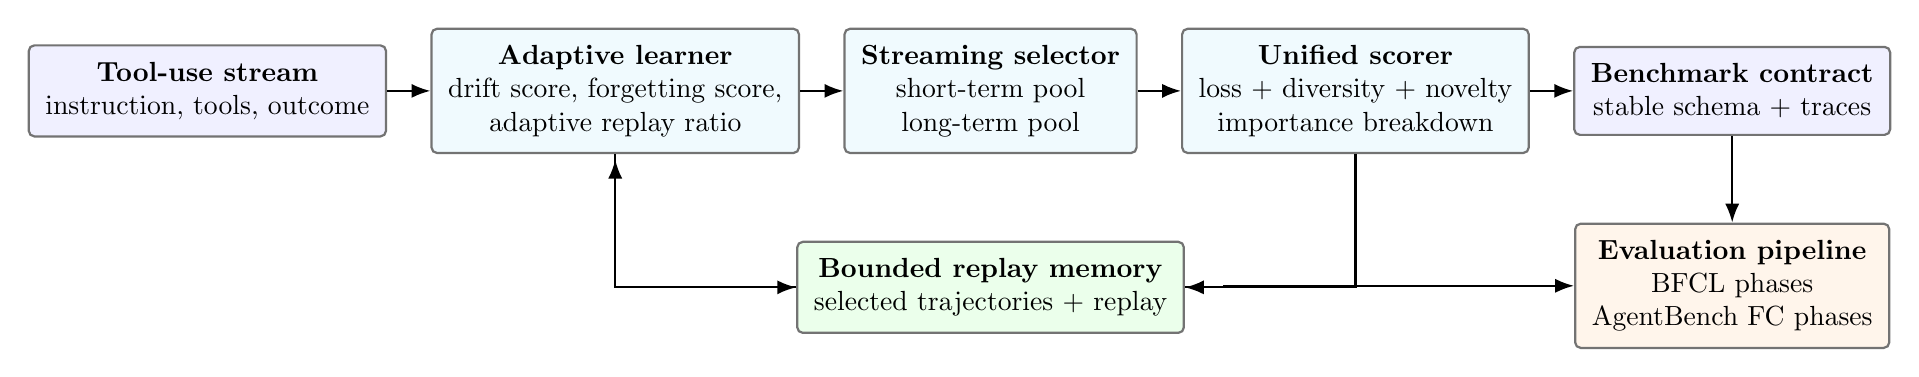
\begin{tikzpicture}[
    node distance=0.55cm and 0.55cm,
    block/.style={draw=black!55, rounded corners=2pt, thick, align=center, minimum height=1.1cm, fill=blue!6, inner sep=6pt},
    wideblock/.style={draw=black!55, rounded corners=2pt, thick, align=center, minimum height=1.2cm, fill=cyan!6, inner sep=6pt},
    arrow/.style={-{Latex[length=2.4mm]}, thick}
]
\node[block, minimum width=2.2cm] (stream) {\textbf{Tool-use stream}\\instruction, tools, outcome};
\node[wideblock, right=of stream, minimum width=3.0cm] (signals) {\textbf{Adaptive learner}\\drift score, forgetting score,\\adaptive replay ratio};
\node[wideblock, right=of signals, minimum width=2.9cm] (selector) {\textbf{Streaming selector}\\short-term pool\\long-term pool};
\node[wideblock, right=of selector, minimum width=3.0cm] (scorer) {\textbf{Unified scorer}\\loss + diversity + novelty\\importance breakdown};
\node[block, right=of scorer, minimum width=2.5cm] (contract) {\textbf{Benchmark contract}\\stable schema + traces};

\draw[arrow] (stream) -- (signals);
\draw[arrow] (signals) -- (selector);
\draw[arrow] (selector) -- (scorer);
\draw[arrow] (scorer) -- (contract);

\node[block, below=1.1cm of selector, minimum width=3.4cm, fill=green!8] (buffer) {\textbf{Bounded replay memory}\\selected trajectories + replay};
\draw[arrow] (signals) |- (buffer);
\draw[arrow] (scorer) |- (buffer);
\draw[arrow] (buffer.west) -| ([yshift=-2pt]signals.south);

\node[wideblock, below=1.1cm of contract, minimum width=3.8cm, fill=orange!8] (bench) {\textbf{Evaluation pipeline}\\BFCL phases \\ AgentBench FC phases};
\draw[arrow] (contract) -- (bench);
\draw[arrow] (buffer.east) -- ++(0.5,0) |- (bench.west);
\end{tikzpicture}
\caption{Code-aligned overview of SIAS. Incoming tool-use experiences are first analyzed by the adaptive learner, which estimates drift and forgetting and adjusts replay behavior. A streaming selector maintains bounded short-term and long-term memory pools, while a unified importance scorer provides a consistent, interpretable criterion for replay and retention. The retained trajectories are exposed through a benchmark-facing contract for BFCL and AgentBench FC evaluation.}
\label{fig:sias_overview}
\end{figure*}

\subsection{Adaptive Replay via Drift and Forgetting Signals}

The learner computes a batch profile from token/topic distributions and observed loss statistics. Given a previous profile and the current batch, SIAS derives:
\begin{itemize}[leftmargin=12pt]
    \item \textbf{drift score}: a normalized combination of topic-shift, token-shift, and batch loss-shift;
    \item \textbf{forgetting score}: the degree to which the current loss exceeds a running historical loss estimate.
\end{itemize}

These signals determine an adaptive replay ratio
\[
r_t = \mathrm{clip}\big(r_0 + \alpha \cdot \max(d_t, f_t),\ r_{\min},\ r_{\max}\big),
\]
where $d_t$ and $f_t$ are the current drift and forgetting scores, and $r_0$ is the base replay ratio.

SIAS further switches among three selection policies:
\begin{itemize}[leftmargin=12pt]
    \item \texttt{loss\_topk}: when forgetting or loss spikes dominate;
    \item \texttt{diversity}: when distributional drift dominates;
    \item \texttt{hybrid}: otherwise.
\end{itemize}

This mechanism is implemented in the current \texttt{OnlineContinualLearner}, which also emits per-round traces including \texttt{drift\_score}, \texttt{forgetting\_score}, \texttt{adaptive\_replay\_ratio}, replay size, and selected IDs.

\subsection{Streaming Coreset Maintenance}

To avoid repeated full recomputation, SIAS uses a streaming selector with two candidate pools:
\begin{itemize}[leftmargin=12pt]
    \item a \textbf{short-term pool} that captures recent arrivals under a sliding replacement policy;
    \item a \textbf{long-term pool} that stores accumulated high-value experiences.
\end{itemize}

Incoming samples first update the short-term pool. The union of short-term and long-term candidates is then ranked by importance, after which the long-term pool is refreshed up to a configured capacity. Final selection for training uses a hybrid of high-score retention and diversity-aware coverage.

This design reduces the need to revisit the entire history after each batch while still preserving coverage over old and new tool-use patterns.

\subsection{Unified Importance Scoring}

A central design principle of SIAS is that replay and coreset selection should not depend on separate, potentially conflicting heuristics. We therefore define a unified importance score
\[
I(x) = \lambda_{\ell} I_{\text{loss}}(x) + \lambda_{d} I_{\text{div}}(x) + \lambda_{n} I_{\text{nov}}(x),
\]
where:
\begin{itemize}[leftmargin=12pt]
    \item $I_{\text{loss}}$ prioritizes samples with high training difficulty or error,
    \item $I_{\text{div}}$ rewards representational coverage relative to other retained samples,
    \item $I_{\text{nov}}$ rewards novelty relative to a reference memory.
\end{itemize}

The implementation stores not only the final score but also an \texttt{importance\_breakdown} for each retained sample. This enables direct debugging and post-hoc analysis of why a trajectory was kept or replayed.

\subsection{Benchmark-Facing Contract and Reproducibility}

SIAS includes a stable benchmark-facing contract with a versioned \texttt{SIASConfig}, fixed input/output schemas, and adapter functions for external callers. Reproducibility is supported by:
\begin{itemize}[leftmargin=12pt]
    \item unified random seed control,
    \item metrics traces in \texttt{metrics.jsonl},
    \item tabular summaries in \texttt{summary.csv},
    \item configuration snapshots in \texttt{config.snapshot.yaml}.
\end{itemize}

These design decisions are not cosmetic. They are necessary for comparing continual-learning variants under identical conditions and for making BFCL / AgentBench FC evaluation reproducible.

\section{Experimental Protocol}

\begin{table*}[t]
\centering
\caption{Planned experimental configuration for the ICML submission. The current repository already implements the SIAS runner and manifest generation for the first four methods; EWC, MIR, and DER++ are the next baselines to be integrated.}
\label{tab:protocol}
\begin{tabular}{p{2.1cm}p{3.2cm}p{3.1cm}p{4.3cm}}
\toprule
\textbf{Axis} & \textbf{Primary Choice} & \textbf{Secondary Choice} & \textbf{Purpose} \\
\midrule
Function-calling benchmark & BFCL & StableToolBench / API-BLEND & Evaluate serial, parallel, and stateful function calling under continual phase splits. \\
Executable environment benchmark & AgentBench FC & Optional WebShop / OS / KG subsets & Measure environment-level task completion and cross-environment retention. \\
Continual-learning baselines & Sequential FT, Fixed Replay, Joint Oracle & EWC, MIR, DER++ & Compare SIAS to lower-bound, upper-bound, replay, and regularization baselines. \\
Main metrics & Success / pass rate, forgetting, FWT, BWT & runtime, memory, sample efficiency & Quantify both effectiveness and systems cost. \\
\bottomrule
\end{tabular}
\end{table*}

\subsection{Primary Benchmark: BFCL}

Our primary benchmark is BFCL \citep{patil2025bfcl}. BFCL is particularly well aligned with our paper because it covers:
\begin{itemize}[leftmargin=12pt]
    \item serial function calls,
    \item parallel function calls,
    \item multi-function settings,
    \item stateful multi-step agentic evaluation.
\end{itemize}

In SIAS, BFCL instances are converted into continual-learning samples using the benchmark adapter in the current repository. We construct continual phases from \texttt{test\_category}, \texttt{category}, or \texttt{domain}, depending on the chosen split protocol.

\subsection{Real Environment Benchmark: AgentBench FC}

Our real environment benchmark is AgentBench FC \citep{agentbenchfc2025}, a function-calling extension of AgentBench that integrates environments such as OS interaction, DBBench, KG, ALFWorld, and WebShop into a unified execution framework. We use AgentBench FC to evaluate whether a continual tool-use learner can preserve prior competence while adapting to new task environments.

AgentBench FC phases are constructed from \texttt{environment} or \texttt{task\_name}. This lets us evaluate not only function-call formatting accuracy but also genuine environment-level task completion and cross-environment transfer.

\subsection{Baselines}

We propose the following baselines:
\begin{itemize}[leftmargin=12pt]
    \item \textbf{Sequential FT}: phase-by-phase fine-tuning without replay;
    \item \textbf{Joint Oracle}: train on all phase data seen so far;
    \item \textbf{ER / Fixed Replay}: uniform or fixed-ratio replay;
    \item \textbf{EWC}: regularization-based retention;
    \item \textbf{MIR or DER++}: strong replay-based continual baselines;
    \item \textbf{SIAS}: adaptive replay + streaming coreset + unified scorer.
\end{itemize}

The current repository already includes manifest generation for \texttt{sequential\_ft}, \texttt{fixed\_replay}, \texttt{sias}, and \texttt{joint\_oracle}. EWC, MIR, and DER++ are the next baselines to be added.

\subsection{Metrics}

We will report:
\begin{itemize}[leftmargin=12pt]
    \item \textbf{Tool-call success / pass rate}: correctness of the function/tool decision;
    \item \textbf{Task completion rate}: environment-level success on AgentBench FC;
    \item \textbf{Forgetting}: degradation on earlier phases after learning later phases;
    \item \textbf{Forward transfer (FWT)} and \textbf{Backward transfer (BWT)};
    \item \textbf{Sample efficiency}: performance as a function of retained/replayed experiences;
    \item \textbf{Runtime and memory overhead}: selector latency, replay cost, and buffer size.
\end{itemize}

\subsection{Result Reporting Template}

Because this manuscript is being aligned to a still-evolving codebase, we explicitly separate \emph{implemented protocol} from \emph{pending full-scale benchmark runs}. To make the paper structurally close to a final submission, Table~\ref{tab:result_template} provides the reporting layout that will be populated after BFCL and AgentBench FC sweeps are completed.

\begin{table}[t]
\centering
\caption{Result reporting template for the final submission. ``TBD'' entries will be filled after full BFCL and AgentBench FC runs.}
\label{tab:result_template}
\begin{tabular}{lcccc}
\toprule
\textbf{Method} & \textbf{Success} & \textbf{Forget} & \textbf{BWT} & \textbf{Cost} \\
\midrule
Sequential FT & TBD & TBD & TBD & TBD \\
Fixed Replay / ER & TBD & TBD & TBD & TBD \\
EWC & TBD & TBD & TBD & TBD \\
MIR / DER++ & TBD & TBD & TBD & TBD \\
SIAS & TBD & TBD & TBD & TBD \\
\bottomrule
\end{tabular}
\end{table}

\subsection{Current Implementation Status}

This draft is intentionally aligned with the implemented repository rather than a hypothetical future system. At the time of writing, the codebase already includes:
\begin{itemize}[leftmargin=12pt]
    \item adaptive replay and reproducibility traces,
    \item streaming coreset selection and benchmark scripts,
    \item unified importance scoring with explanations,
    \item benchmark-facing contracts and integration tests,
    \item BFCL / AgentBench FC experiment manifest generation.
\end{itemize}

The remaining empirical work is to run full BFCL and AgentBench FC sweeps, add EWC/MIR/DER++ runners, and populate the final result tables and figures. We emphasize this status explicitly because the goal of this draft is to be \emph{review-ready in structure} while staying faithful to what is already implemented.

\section{Discussion and Limitations}

SIAS currently optimizes the algorithm layer for continual tool use, but several limitations remain.

\paragraph{Empirical results are not yet fully populated.}
The repository already supports ablation scripts, contract tests, and real-data manifest generation, but the final ICML-ready benchmark tables still require long-run BFCL and AgentBench FC evaluation.

\paragraph{The current benchmark adapters are generic.}
Our BFCL and AgentBench FC adapters are designed to ingest local JSON / JSONL data with robust key matching. For the final paper, these adapters should be tightened to the exact public release schemas of the selected benchmark versions.

\paragraph{Classical continual baselines still need to be integrated.}
While SIAS already supports sequential, fixed replay, joint oracle, and its own adaptive policy, the strongest reviewer-expected baselines (e.g., EWC, MIR, DER++) still need to be instantiated in the benchmark runner.

\paragraph{Tool-use continual learning is broader than function calling.}
BFCL and AgentBench FC are a strong starting point, but longer-term settings may require richer environment-level curricula, tool insertion/removal schedules, and dynamic schema evolution.

\section{Conclusion}

We presented SIAS, a streaming importance-aware framework for continual agent tool use. SIAS unifies three implemented ideas---adaptive replay from drift and forgetting signals, streaming coreset maintenance under bounded memory, and a unified importance score shared by replay and retention decisions---within a benchmark-facing continual-learning stack. Rather than treating tool use and continual learning as separate evaluation tracks, SIAS explicitly targets their intersection and grounds that goal in the two benchmarks most relevant to the setting: BFCL and AgentBench FC. The repository already provides the algorithmic core, reproducibility infrastructure, and real-dataset experiment scaffolding required for a full empirical study. The next step is to complete large-scale benchmark sweeps against replay and regularization baselines and to translate those runs into the final ICML submission tables and figures.

\bibliography{references}
\bibliographystyle{icml2025}

\appendix
\section{Draft Positioning}

This version is intentionally written as a \emph{formal anonymous ICML draft} rather than an internal design memo. The method, protocol, and software stack are real and implemented; the missing component is the final large-scale benchmark execution. We preserve that distinction explicitly to avoid overstating the empirical state of the project while still making the paper structurally close to a submission-ready manuscript.

\section{Implemented Repository Components}

The current repository contains the following modules directly related to this paper draft:
\begin{itemize}[leftmargin=12pt]
    \item \texttt{src/sage\_sias/continual\_learner.py}: adaptive replay, drift/forgetting signals, reproducibility traces;
    \item \texttt{src/sage\_sias/coreset\_selector.py}: hybrid and streaming coreset selection;
    \item \texttt{src/sage\_sias/importance\_scorer.py}: loss/diversity/novelty importance scoring;
    \item \texttt{src/sage\_sias/contract.py}: benchmark-facing contract v1;
    \item \texttt{src/sage\_sias/experiment\_framework.py}: BFCL and AgentBench FC dataset adaptation and manifest generation.
\end{itemize}

\section{Planned Result Tables}

The final paper will include at least the following result blocks:
\begin{enumerate}[leftmargin=14pt]
    \item BFCL continual evaluation under category/domain phases;
    \item AgentBench FC continual evaluation under environment phases;
    \item SIAS ablations: no replay, fixed replay, dynamic replay, no coreset, batch coreset, streaming coreset, no unified scorer;
    \item runtime and memory cost analysis;
    \item sample efficiency and forgetting curves.
\end{enumerate}

\end{document}
